\subsubsection{Hipóteses inicias}
\label{initial-hypotheses}

Vamos considerar que no início da epidemia $S \approx 1$. Com essa aproximação e restringindo o modelo para as equações de $E, I, A$ e $T$, temos um sistema com quatro equações lineares \eqref{initial-system}, cuja solução é combinação linear de exponenciais.  
Podemos assumir que a testagem diária no início da pandemia era de $\rho \approx 0$ e, como já mencionado na sessão anterior, os parâmetros $\gamma_1, \tau$ e $\sigma$ são conhecidos. Os parâmetros $\alpha$ e $\beta$ são fixos no período. 

\begin{equation}
    \begin{bmatrix}
        \dot{E} \\ \dot{I} \\ \dot{A} \\ \dot{T} 
    \end{bmatrix} = 
    \begin{bmatrix}
        - \tau & \beta & \beta & 0 \\
        \tau & -\sigma & 0 & 0 \\
        0 & \sigma \alpha & -\gamma_1 & 0 \\
        0 & \sigma (1 - \alpha) & 0 & 0  
    \end{bmatrix}\cdot
    \begin{bmatrix}
        E \\ I \\ A \\ T 
    \end{bmatrix} 
    \label{initial-system}
\end{equation}

O valor $T(-14)$ corresponde aos dados de confirmados em 2 de março e $T(-15) = 0$.  
Assim estimamos $\theta_0 = (\alpha, \beta, E(-14), I(-14), A(-14))$ de forma a minimizar a expressão pgf
\begin{equation}
    \sum_{i=-14}^{0} w_i\left(y_i^{(1)} - \hat{T}(i, \theta_0)\right)^2,
\end{equation}
em que $w_i = \dfrac{i+14}{14}$. Com essas estimativas, obtemos os valores $(E(0), I(0), A(0))$ que determinam o início da pandemia. 
Não há mortes no início da pandemia, o que permite colocar $\mu = 0$. 
Usando que $R(-14) = 0$, obteremos que $Q(-14) = T(-14)$ e, assim, podemos integrar as curvas $Q$ e $R$ até obter os valores $Q(0)$ e $R(0)$. 
Por fim $S(0) = 1 - E(0) - I(0) - A(0) - Q(0) - R(0)$.

\subsubsection{Método de estimação}
\label{estimation-method}

Utilizaremos o método de {\em mínimos quadrados ponderados} para estimar os parâmetros desconhecidos, considerando a observação de casos confirmados e mortes diárias como indicado nas equações \eqref{obsT} e \eqref{obsD}. 
Nessa abordagem, resolvemos um problema de minimização não linear com restrições e a cada iteração integramos o sistema de equações diferenciais. Definimos a função objetivo como:
\begin{gather}
\label{objective}
    F(\theta) = (y^{(1)} - \hat{T}(\theta))^T\Sigma^{-1}(y^{(1)} - \hat{T}(\theta)) + \psi(y^{(2)} - \hat{T}(\theta))^T\Sigma^{-1}(y^{(2)} - \hat{D}(\theta)) 
\end{gather}
tal que $\hat{T}(\theta)$ e $\hat{D}(\theta)$ são os vetores soluções
numéricas das equações diferenciais através do método Runge-Kutta,
$\sigma_k^2\Sigma$ é a matriz de covariância dada pela equação
\eqref{cov-matrix} ($k=1,2$) e $\psi$ é um peso de importância das mortes na
minimização e está relacionado à razão das variâncias $\sigma_1^2/\sigma_2^2$.
A escolha dessa função está relacionada com as propriedades estatísticas dos
dados. Sabemos que, pela hipótese de normalidade, minimizar a
expressão \ref{objective} é equivalente a maximizar a verossimilhança. 
Utilizamos o algoritmo L-BFGS-B \cite{byrd1995}, baseado no método de projeção gradiente e no algoritmo BFGS com uso limitado de memória computacional, implementado na biblioteca Scipy \cite{scipy} da linguagem de programação Python e o código está disponível no Github \cite{github}. 

\subsubsection{Análise residual e \texorpdfstring{$\mathcal{R}_t$}{Rt}
estimado}
\label{residual-analysis}

Escolhemos, de modo arbitrário, fixar a data final para análise dos dados em 31 de julho de 2020 e primeiro ajustamos a curva aos dias iniciais da epidemia, conforme explicado na Seção \ref{initial-hypotheses}. 
Obtemos o resultado na Figura \ref{Fig:initial-values}. 
Definindo a priori $\psi = 119.57$ (valor aproximado entre as variâncias dos dados de casos e óbitos) e os hiperparâmetros ligados à otimização, como os limites superior e inferior e chutes iniciais de cada parâmetro, vamos analisar os resíduos do ajuste de dados e o $\mathcal{R}_t$ induzido pela estimação dos parâmetros segundo: 
\begin{enumerate}
    \item[(i)] o número de coeficientes a serem estimados para $\beta$ e $\mu$; e 
    \item[(ii)] a ordem das B-splines para os parâmetros $\beta$ e $\mu$.
\end{enumerate}

\begin{figure}
    \centering
    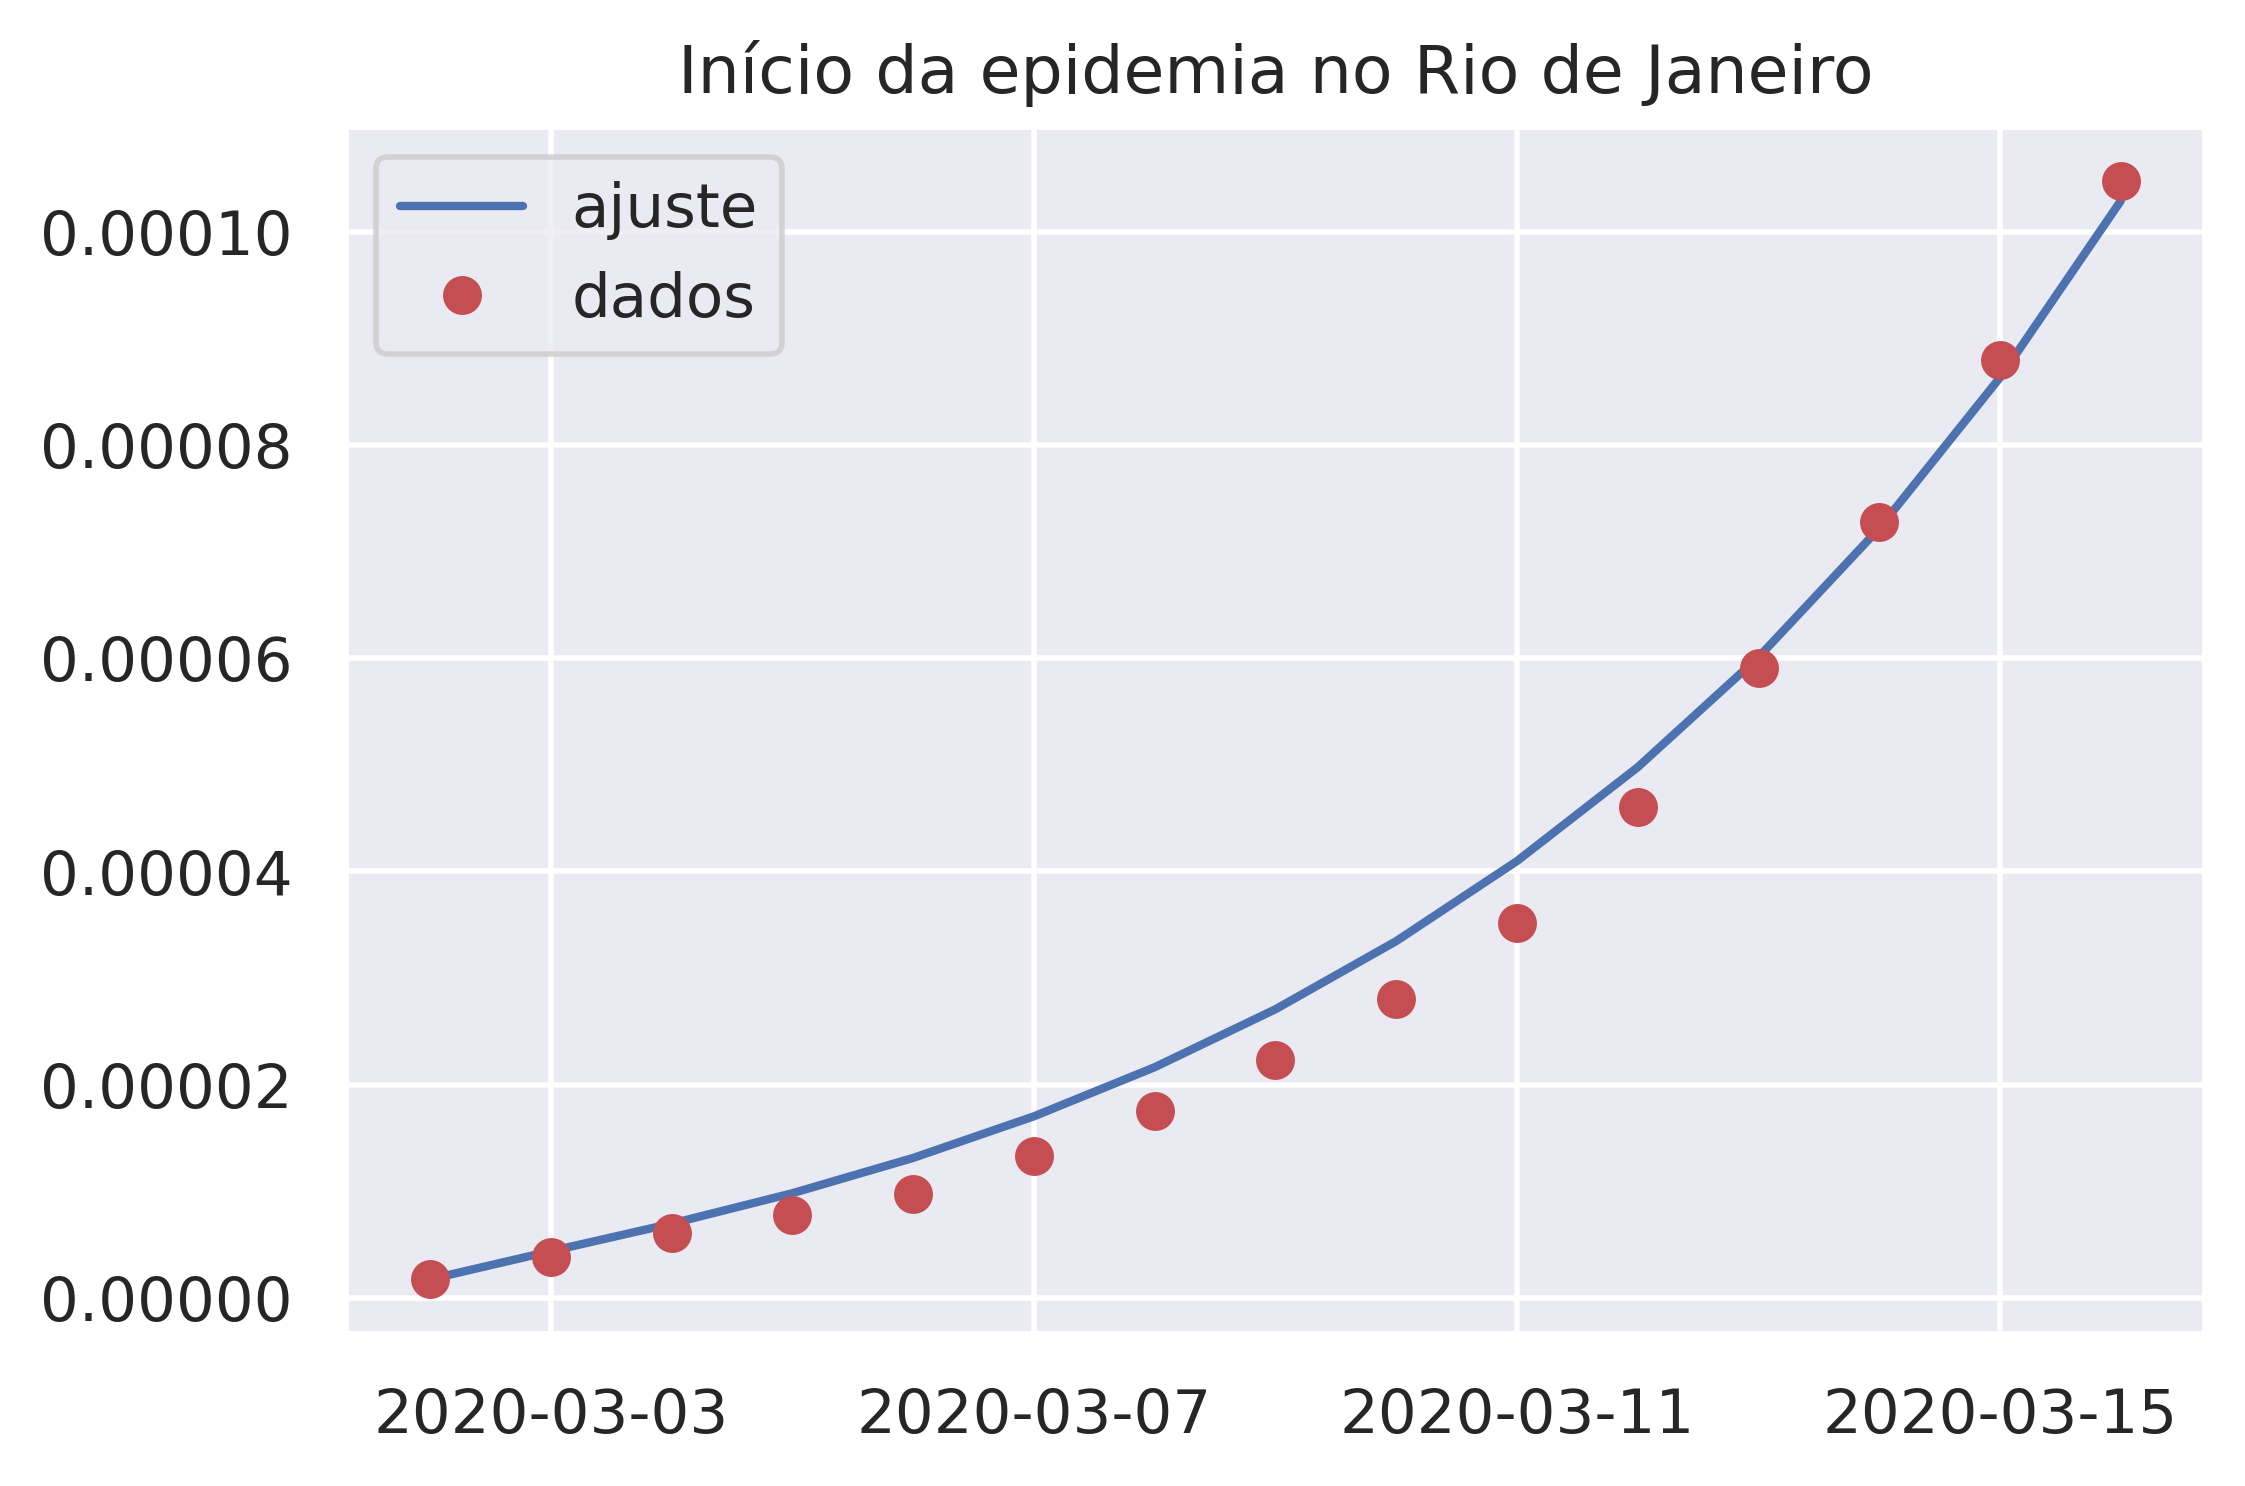
\includegraphics[width=0.5\textwidth]{../images/initial_values.png}
    \caption{Ajuste à curva acumulada de casos no início da epidemia para obtenção dos valores iniciais, como explicado na Seção \ref{initial-hypotheses}.}
    \label{Fig:initial-values}
\end{figure}

Por exemplo, colocando 4 coeficientes para as B-splines de ordem 3 para ambos
os parâmetros que variam no tempo, obtemos as curvas
descritas na Figura \ref{Fig:cumulated-curves}. Em particular $\alpha$ foi estimado em 0.899. 

\begin{figure}[H]
    \centering
    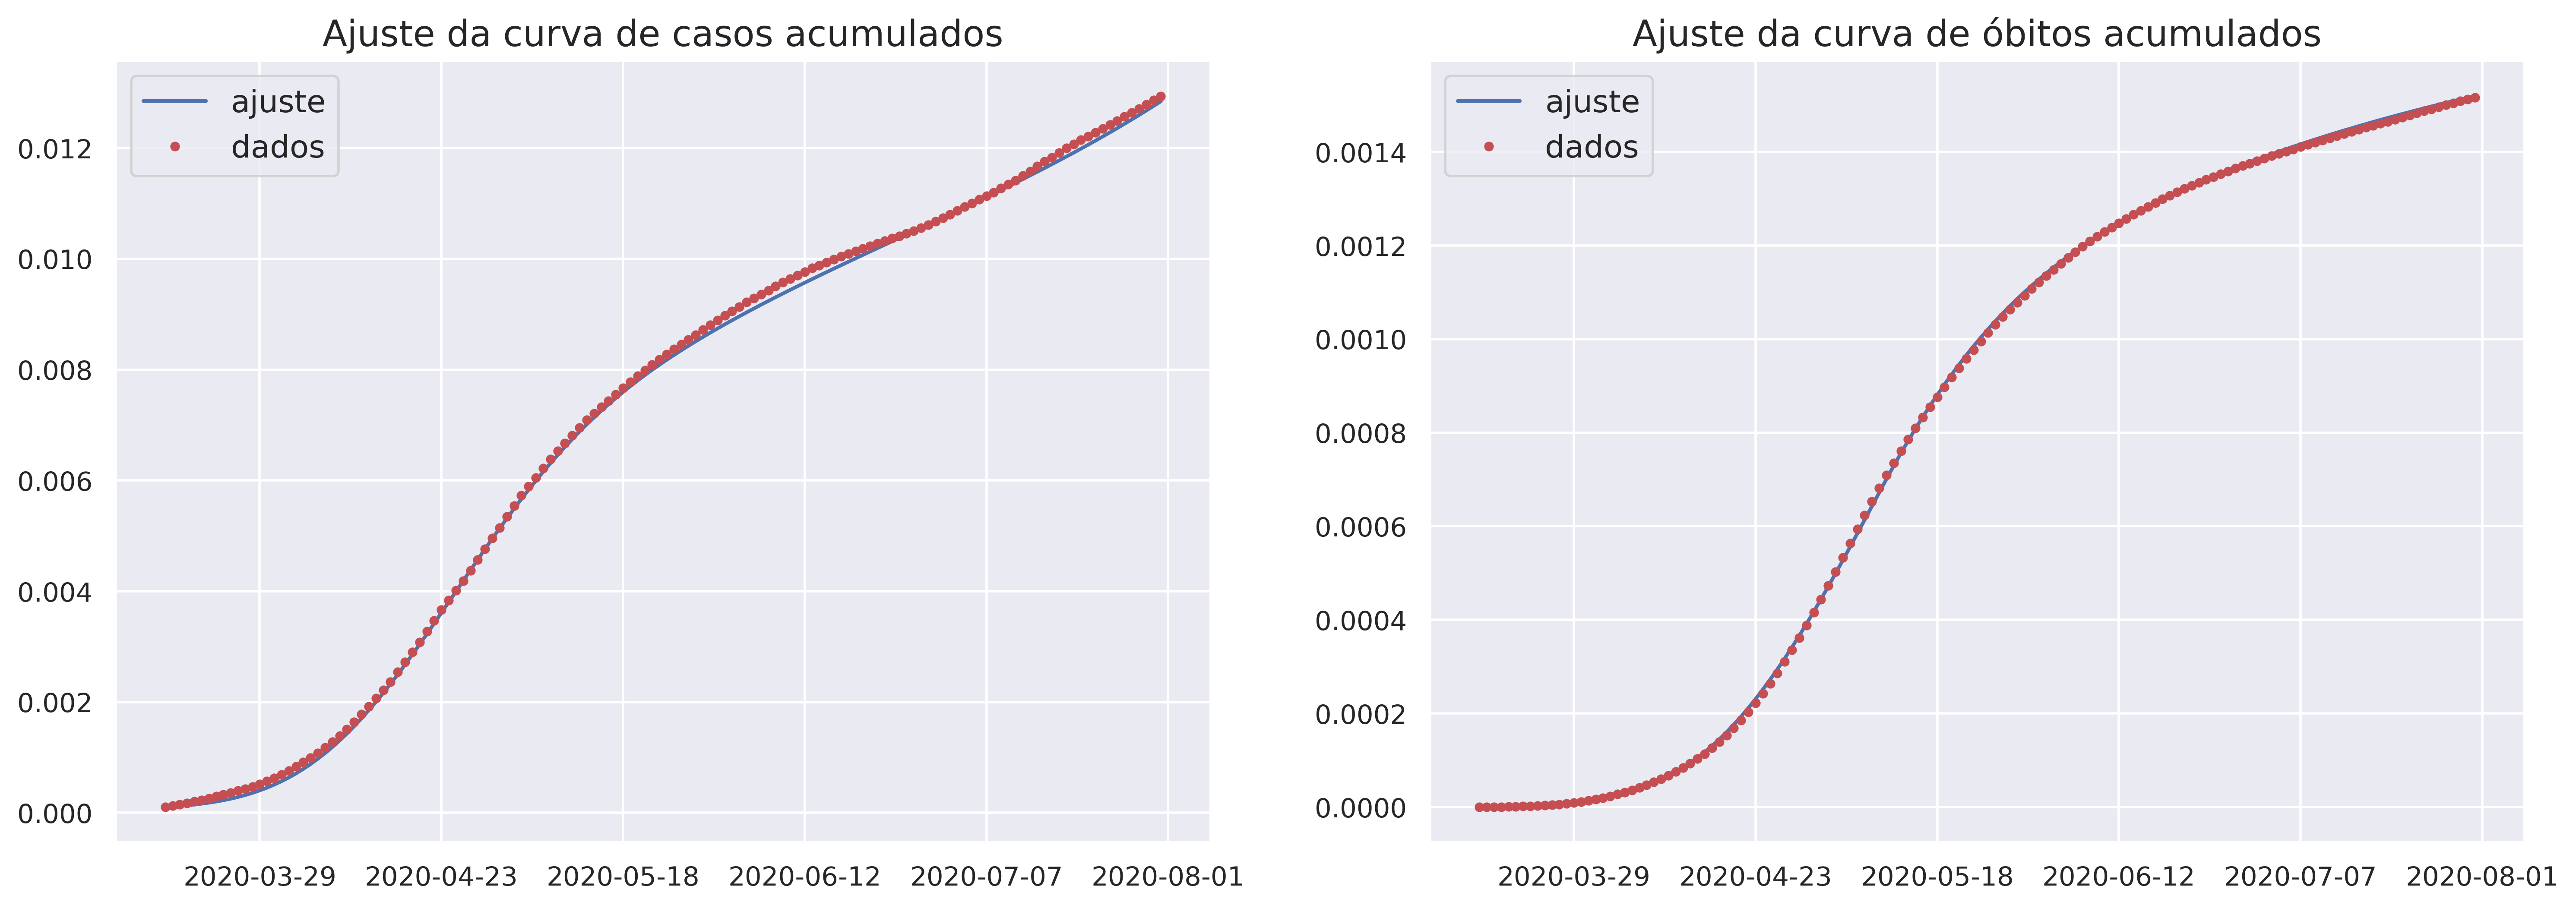
\includegraphics[width=\textwidth]{../images/cumulated_fitted_curves.png}
    \caption{Ajuste das curvas acumuladas de casos e óbitos, respectivamente.}
    \label{Fig:cumulated-curves}
\end{figure}

Com esse resultado, podemos verificar se os resíduos do modelo aproximam os erros, que por hipótese têm distribuição Gaussiana. 
Primeiro diferenciamos para obter resíduos diários, de forma que sua variância seja constante (ver equações \eqref{obsT1} e \eqref{obsD1}) e, então, desenhamos os {\em histogramas} (indicador da frequência de cada resíduo) e os {\em gráficos Q-Q} (comparação dos quartis da distribuição Gaussiana com os quartis da distribuição amostral dos resíduos) que são apresentados na Figura
\ref{Fig:check_residuals}. 
Já visualizamos que ambas as curvas não têm um ajuste com resíduos como esperado, principalmente a curva de mortes. 
Além dessa análise visual, também podemos aplicar testes estatísticos  para verificar correlação e normalidade.  

O {\em teste Ljung-Box} \cite{ljung1978} é um teste estatístico que verifica a autocorrelação em uma série temporal, cuja hipótese nula afirma que as k-correlações são nulas, isto é, a série temporal é independentemente distribuída. 
Aplicando-o nos resíduos do ajuste para as duas curvas, obtivemos o p-valor 0 computacional, o que indica que os resíduos não são descorrelacionamos como assumimos. 
Já o {\em teste Jarque-Bera} \cite{jarque1980} avalia a assimetria e a curtose da distribuição amostral e compara com as da normal.
No nosso caso, a hipótese nula não foi rejeitada à nível 5\%, o que é um bom indicativo de normalidade dos resíduos. 
Concluímos, em particular, que o modelo, apesar de um ajuste interessante, com resíduos normalmente distribuídos, tem resíduos correlacionados, o que precisa ser melhor estudado em trabalhos futuros. 
Podemos fazer essa análise para todas as combinações de parâmetros que desejarmos. 
Para mais detalhes, confira no Github \cite{github}.

\begin{figure}
    \centering
    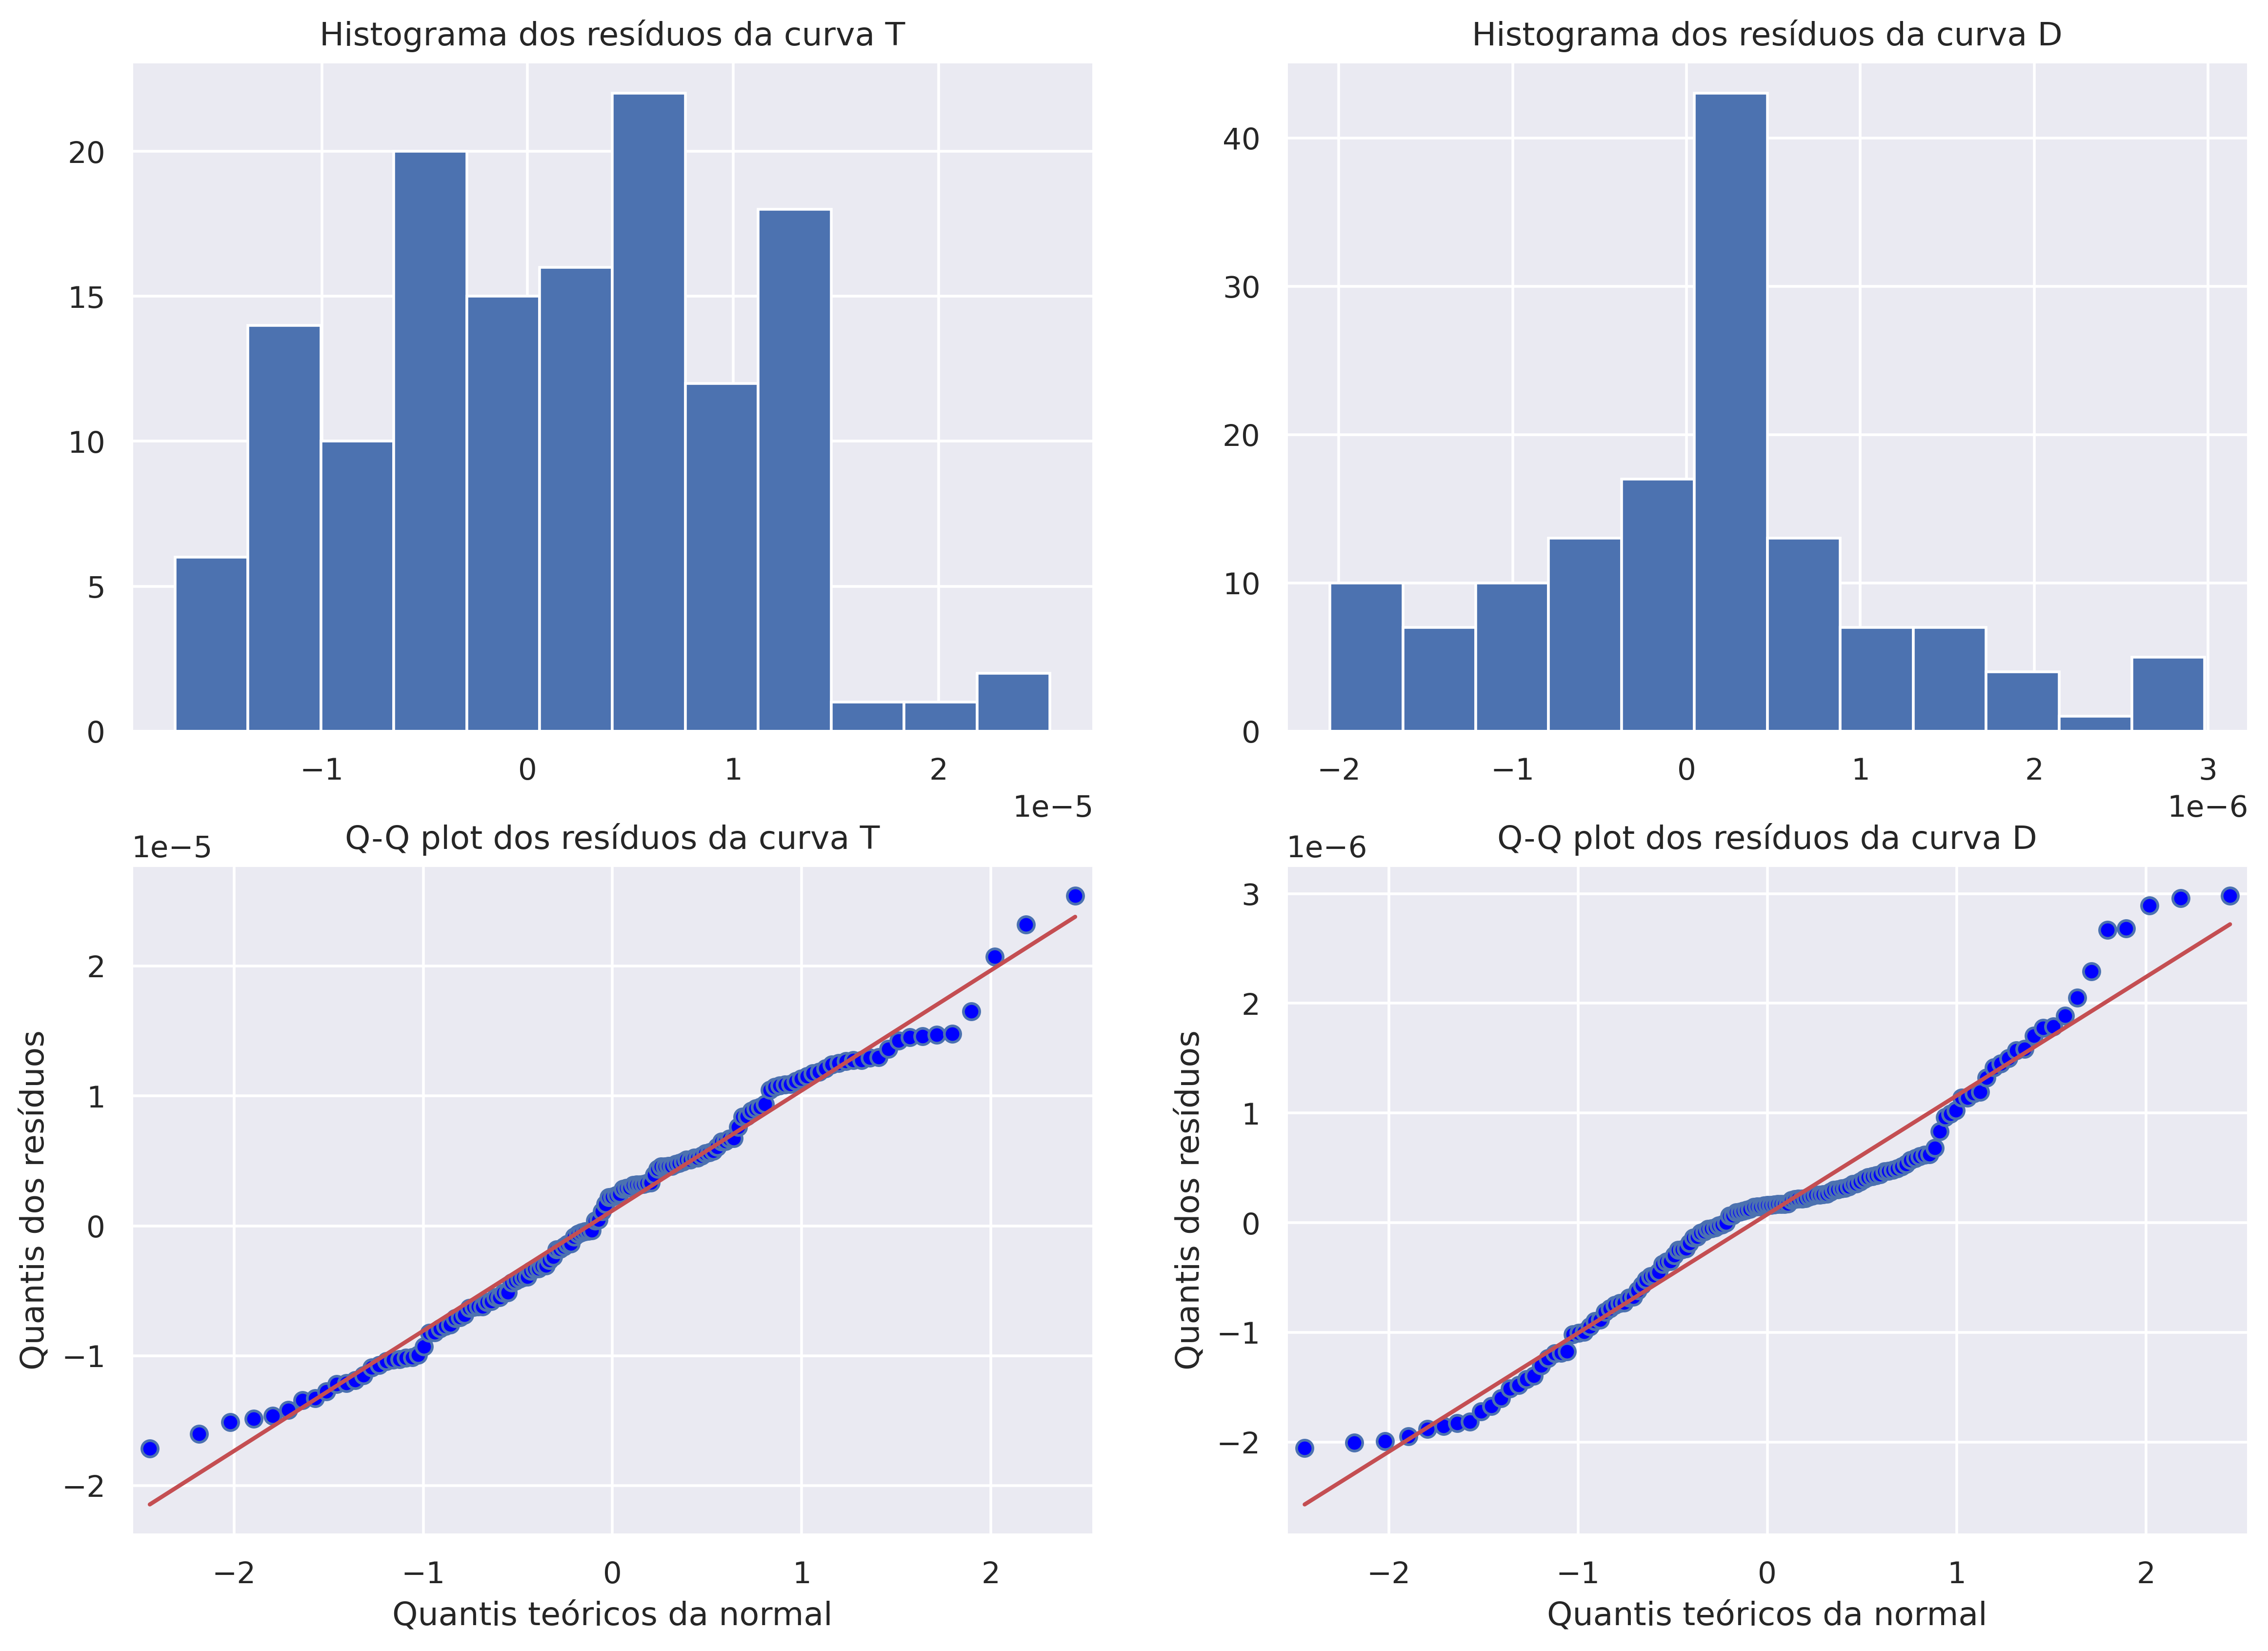
\includegraphics[width=.8\textwidth]{../images/check_residuals.png}
    \caption{Análise gráfica dos resíduos com histograma e Q-Q plot.}
    \label{Fig:check_residuals}
\end{figure}

Outra característica importante a ser analisada é o número reprodutivo básico,
descrito na Seção \ref{sec:R0}. Para os parâmetros estimados no exemplo,
obtemos o $\mathcal{R}_t$ descrito na Figura \ref{Fig:rt_modelo}. 
Considerando as estimativas do $\mathcal{R}_0$ para o Brasil em
\cite{rtBrasil2020}, encontramos no dia 23 de março o valor de 2.325
para o modelo SIRD, e 2.897 para o modelo SIRASD. Em
\cite{rt-imperial-college}, a estimativa pontual para o dia 9 de maio de 2020
do estado do Rio de Janeiro foi de $1.1$ com 95\%-intervalo de confiança
$[0.9, 1.3]$ , que inclui nosso valor. Por fim, a curva estimada por
\cite{observatorio} para a cidade do Rio de Janeiro tem um formato muito
similar à da Figura \ref{Fig:rt_modelo}, em que no começo de maio, o $\mathcal{R}_t$ tem estimativa menor do que 1 e
volta a crescer até ficar maior do que 1 no final de julho. Esses valores corroboram nossa estimação. 

\begin{figure}[!ht]
    \centering
    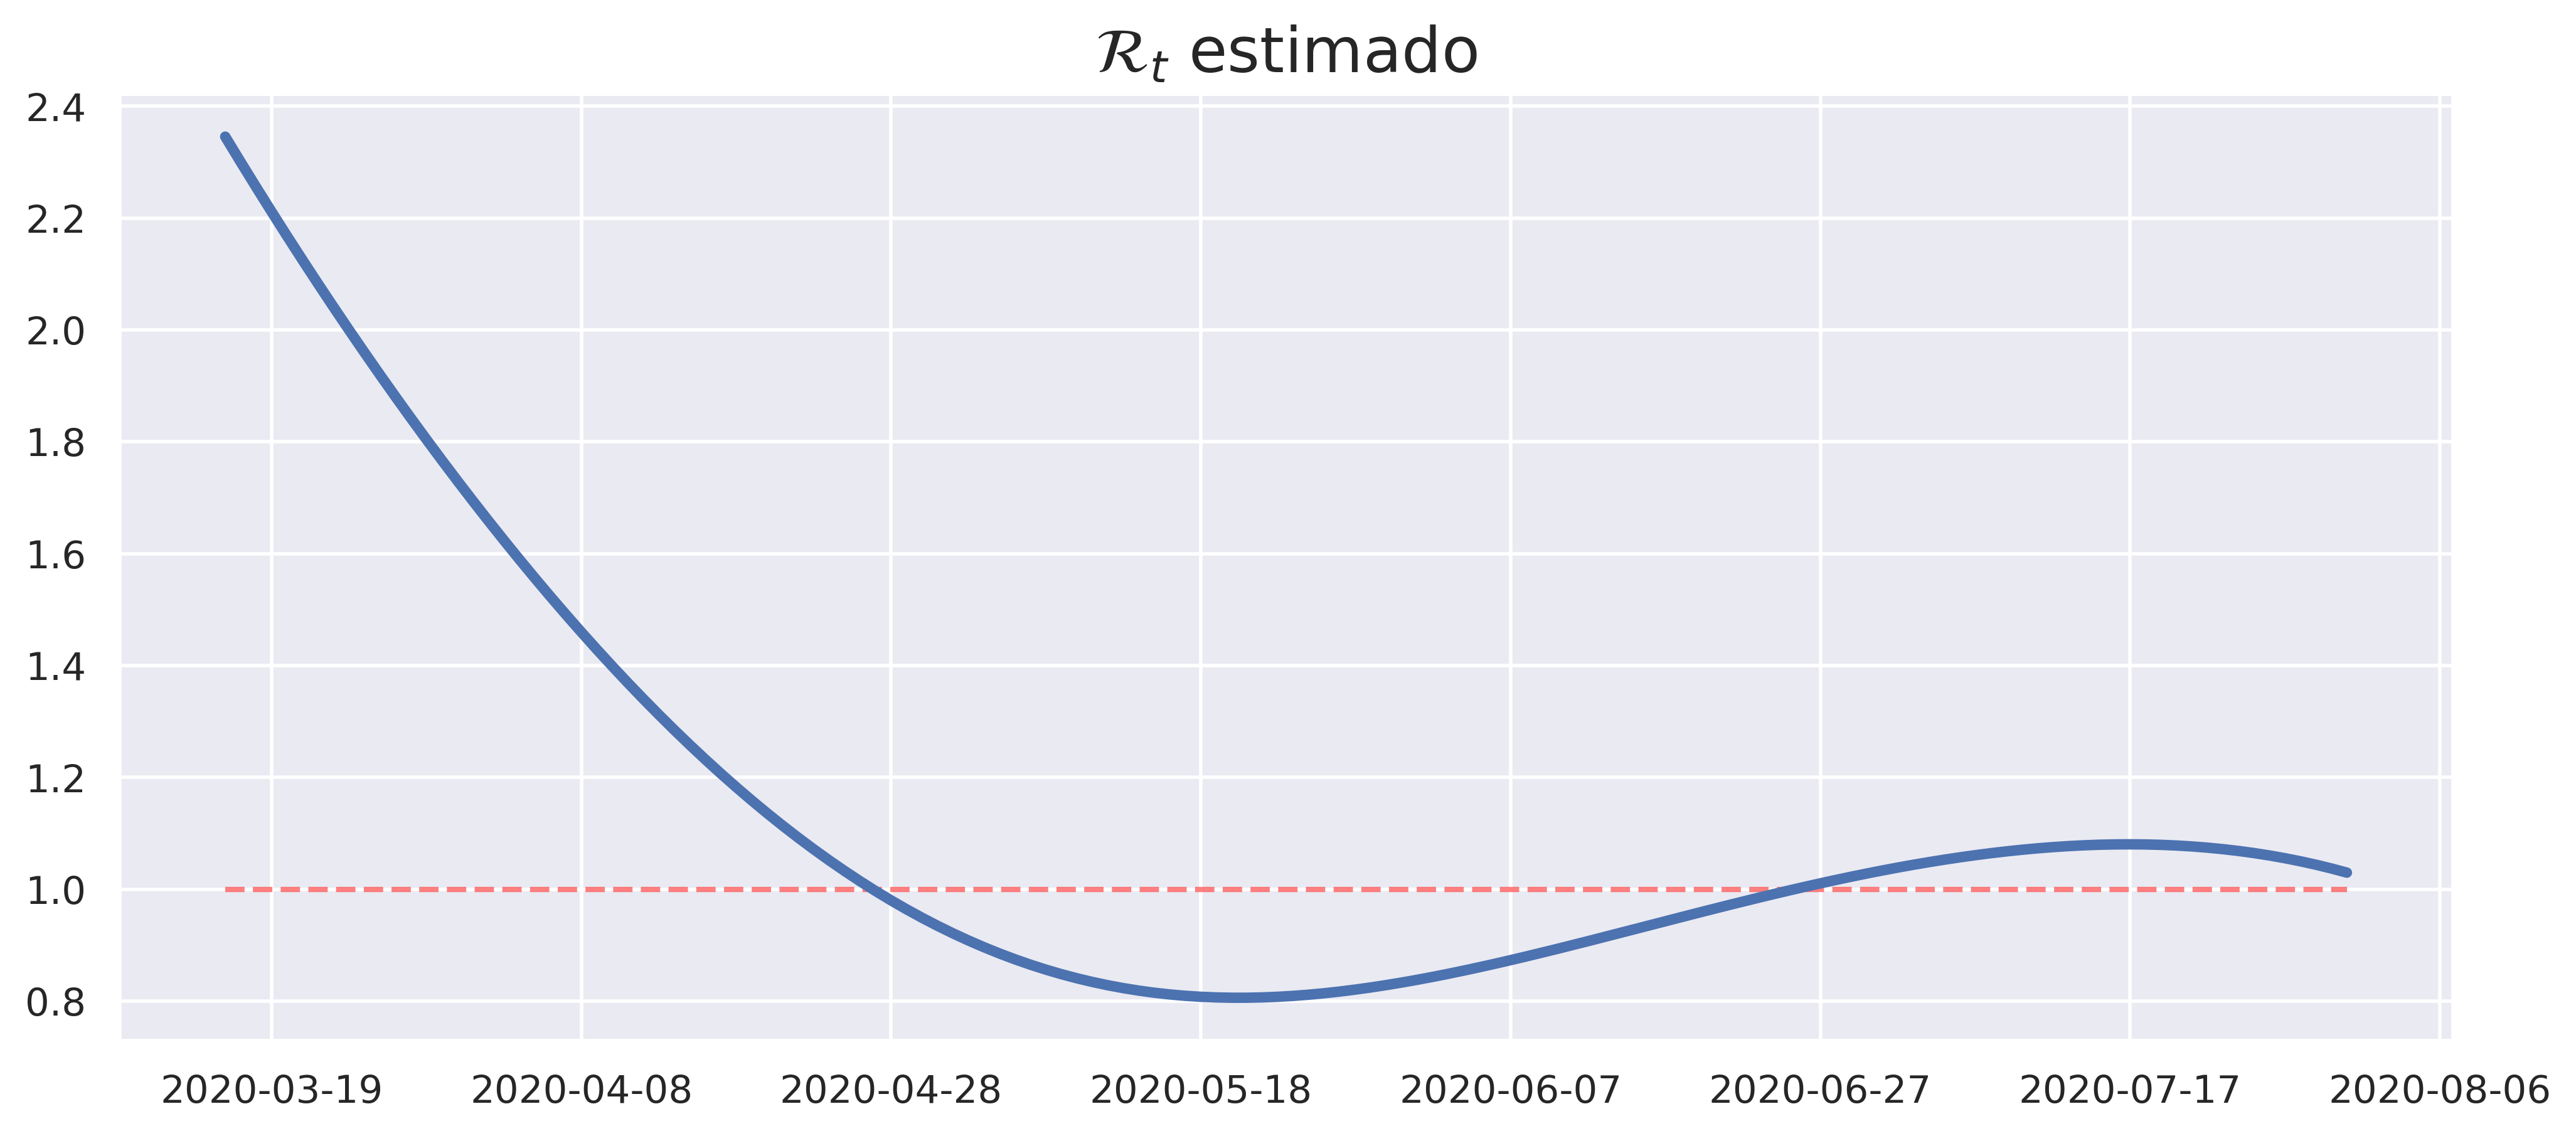
\includegraphics[width=0.8\textwidth]{../images/rt_example.png}
    \caption{Número reprodutivo ao longo do primeiros cinco meses de pandemia para os parâmetros do exemplo.}
    \label{Fig:rt_modelo}
\end{figure}

Para determinar a ordem $r$ e $s$, e o número de coeficientes para a aproximação por B-splines, usamos o {\em critério de informação AIC} descrito em \cite{liang2010}, que sob a hipótese de normalidade dos erros, pode ser calculado segundo a fórmula 
\begin{equation}
    AIC = n\ln\left(\frac{RSS}{n}\right) + 2K, 
\end{equation}
onde $K$ é o número de parâmetros desconhecidos e $RSS$ é a soma dos quadrados dos resíduos do modelo. Os resultados podem ser conferidos na Tabela \ref{Tab:aic-comparison}. 
Para esse experimento, escolhemos comparar modelos com 3 e 4 coeficientes, pois modelos com menos do que 3 coeficientes se mostrarem incapazes de capturar a variação temporal, enquanto modelos com mais do que 4 parâmetros são difíceis de estimar. 
Com isso, a ordem das splines pode variar de $k = 0$ a $k = \text{número de coeficientes} - 1$. 

\begin{table}[ht]
    \centering
    \begin{tabular}{|l|c|c|c|c|c|c|c|c|}
    \hline
    \multicolumn{2}{|c|}{\multirow{2}{*}{B-splines}}                       &
    \multicolumn{7}{|c|}{Parâmetros $\mu$}
    \\ \cline{3-9} 
    \multicolumn{2}{|c|}{}                                        & \textbf{(3,0)} & \textbf{(3,1)} & \textbf{(3,2)} & \textbf{(4,0)} & \textbf{(4,1)} & \textbf{(4,2)} & \textbf{(4,3)} \\ \hline
    \multirow{7}{*}{\rotatebox[origin=c]{90}{Parâmetros $\beta$}} & \textbf{(3,0)} & -2.021        & -2.029         & -2.023         & -2.025         & -2.028         & -2.032         & -2.001        \\ \cline{2-9} 
    & \textbf{(3,1)} & -2.228         & -2.241         & -2.266         & -2.288         & -2.298         & -2.311         & -2.298           \\ \cline{2-9} 
    & \textbf{(3,2)} & -2.246         & -2.230         & -2.253         & -2.294         & -2.337         & -2.331         & -2.309         \\ \cline{2-9} 
    & \textbf{(4,0)} & -1.967         & -1.979         & -1.979         & -1.998         & -2.002         & -2.000         & -1.987         \\ \cline{2-9} 
    & \textbf{(4,1)} & -2.262         & -2.304         & -2.277         & -2.302         & -2.372         & -2.348         & -2.338         \\ \cline{2-9} 
    & \textbf{(4,2)} & -2.346         & -2.243         & -2.262         & -2.300         & -2.374         & -2.357         & -2.332         \\ \cline{2-9} 
    & \textbf{(4,3)} & -2.213         & -2.233         & -2.251         & -2.294         & -2.363         & -2.347         & -2.323         \\ \hline
\end{tabular}
    \caption{Seleção de modelo segundo o AIC (escala $10^3$): os parâmetros que variam no
    tempo aproximados por 3 ou 4 parâmetros e ordem de 0 ao número
    de coeficientes - 1.}
    \label{Tab:aic-comparison}
\end{table}

Segundo o critério, o modelo escolhido possui 4 coeficientes para os dois parâmetros, com ordem das B-splines 2 para $\beta$ e 1 para $\mu$. 
Os resultados para o modelo escolhido não são muito diferentes dos gráficos já apresentados, incluindo a estimação de $\alpha = 0.898$ e podem ser conferidos no Github.

\subsubsection{Identificabilidade prática}
\label{identificability-practical}

O processo de identificabilidade estrutural desenvolvido na Seção \ref{identificability} é feito com base em duas hipóteses: a estrutura do modelo é precisa e os erros de mensuração são ausentes. 
Essas hipóteses não são válidas na prática e, por isso, é necessário avaliar se os parâmetros podem ser estimados de forma confiável e com precisão a partir dos dados ruidosos \cite{miao2011}. 
Seja $\hat{\theta} = (\hat{\alpha}, \hat{\beta}_1, ...,\hat{\mu}_{r})$ o vetor de estimativas a partir do ajuste aos dados. 
A {\em matriz de correlação} é um método que examina as correlação entre os parâmetros do modelo e pode ser calculada com base na {\em matriz Informação de Fisher (FIM)} da seguinte maneira, 
\begin{equation}
    FIM = \frac{1}{\hat{\sigma}_1^2}\left(\frac{\partial \hat{T}}{\partial \theta}\right)\Bigg|_{\theta = \hat{\theta}}^{T}\Sigma^{-1}\left(\frac{\partial \hat{T}}{\partial \theta}\right)\Bigg|_{\theta = \hat{\theta}} + \frac{1}{\hat{\sigma}_2^2}\left(\frac{\partial \hat{D}}{\partial \theta}\right)\Bigg|_{\theta = \hat{\theta}}^{T}\Sigma^{-1}\left(\frac{\partial \hat{D}}{\partial \theta}\right)\Bigg|_{\theta = \hat{\theta}}
    \label{fim}
\end{equation}
e a {\em matriz de covariâncias} $C$ é igual a inversa de $FIM$ (equação \eqref{fim}). Finalmente, o elemento $r_{ij}$, $1 \le i,j \le r + s + 1$ da {\em matriz de correlações} pode ser definido como 
\begin{equation}
    r_{ij} = \frac{C_{ij}}{\sqrt{C_{ii}C_{jj}}}
    \label{correlation}
\end{equation}
que mensura a correlação entre as estimativas $\hat{\theta}_i$ e $\hat{\theta}_j$. 
Uma correlação próxima a 1 indica que os parâmetros são praticamente indistinguíveis e um depende fortemente do outro. 
Em particular, ao calcularmos $R = [r_{ij}]$ para os parâmetros estimados, obtemos uma uma matriz de dimensão $K \times K$ onde $K$ é o número de parâmetros. 
Podemos visualizar através de um mapa de calor na Figura \ref{fig:corr-matrix} que $\alpha$ e o segundo coeficiente da B-spline de $\beta$ são fortemente correlacionados, mas negativamente. Isso não é um bom sinal quando se trata de identificabilidade.

\begin{figure}[!hb]
    \centering
    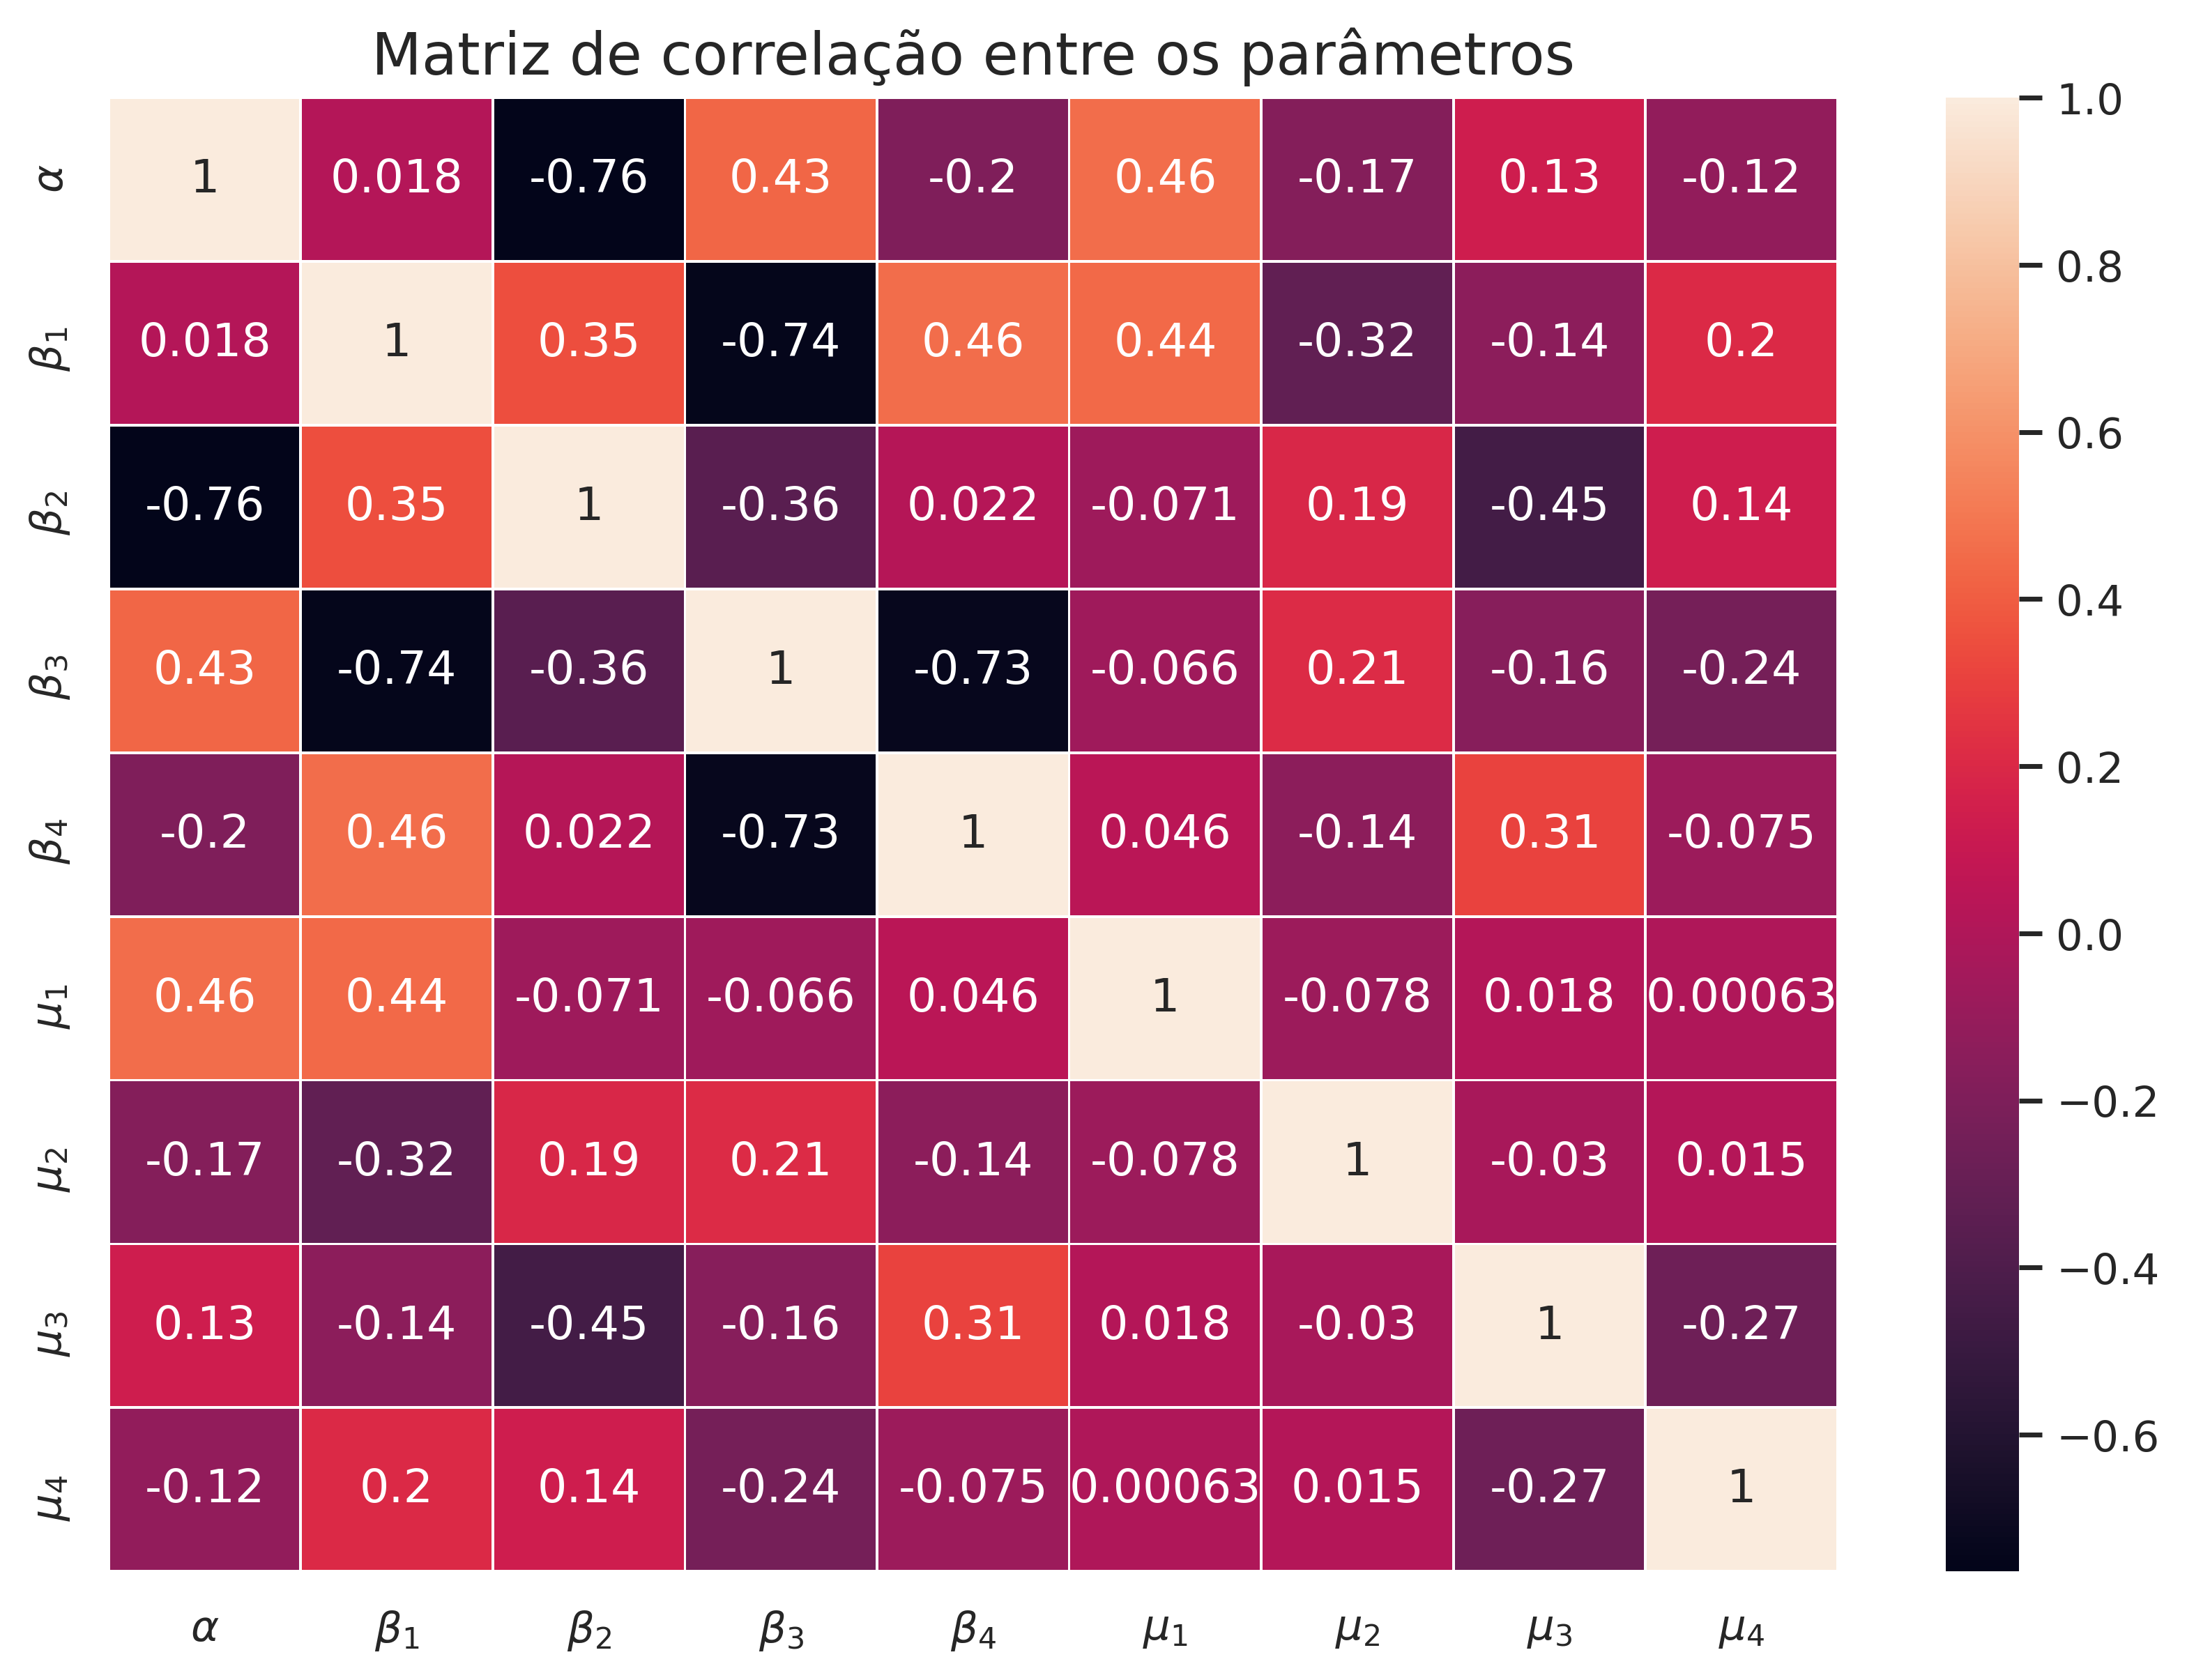
\includegraphics[width=0.8\textwidth]{../images/correlation_matrix.png}
    \caption{Matriz de correlação dos parâmetros estimados do modelo.}
    \label{fig:corr-matrix}
\end{figure}

Outra questão que pode ser levantada é sobre a influência da escolha dos parâmetros epidemiológicos, isto é, se eles variassem um pouco, o quanto isso afetaria a estimação de $\alpha$. 
Para fazer essa análise, escolhemos uma rede de valores para cada parâmetro baseada nos intervalos de confiança estimados nos respectivos artigos citados na Tabela \ref{tab:parameter_values}, estimamos os parâmetros do modelo e reportamos os menores intervalos que englobam os
valores estimados de $\alpha$ (com precisão até a terceira casa decimal), que podem ser conferidos na Tabela\ref{tab:range-parameters}. 
A fixação dos parâmetros influi pouco na estimação final de $\alpha$, portanto. 

\begin{table}[!hb]
    \centering
    \begin{tabular}{|c|c|c|}
    \hline
    \textbf{Parâmetro} & \textbf{Intervalo} & \textbf{Faixa de valores de $\alpha$} \\ \hline
    $\tau^{-1}$        & $[2,4]$            & $[0.897,0.902]$                       \\ \hline
    $\sigma^{-1}$      & $[2,4.5]$          & $[0.897, 0.9]$                         \\ \hline
    $\rho$             & $[0,10^{-4}]$      & $[0.898, 0.899]$                               \\ \hline
    $\gamma_1^{-1}$    & $[6.5,9.5]$        & $[0.894, 0.903]$                       \\ \hline
    $\gamma_2^{-1}$    & $[11,16]$          & $[0.896, 0.898]$                       \\ \hline
    \end{tabular}
    \caption{Rede de valores dos parâmetros fixados e o menor intervalo que inclui os valores estimados de $\alpha$}
    \label{tab:range-parameters}
\end{table}